\chapter{METODOLOGIA}{}
\section{Sistema Proposto}

O sistema proposto neste trabalho consiste no desenvolvimento de uma estação de aquisição de dados elétricos, capaz de monitorar grandezas como corrente e tensão em tempo real, utilizando uma plataforma embarcada de baixo custo voltada para ambientes residênciais. Além disso, propoem-se a realização de um pós processamento desses dados coletados, com o objetivo de analisar e prever o consumo de energia elétrica por meio de técnicas de aprendizado de máquina.

A arquitetura do sistema é centrada no microcontrolador Raspberry Pi Pico 2 W, responsável pela aquisição, processamento, armazenamento e exibição dos dados coletados. Para a medição de corrente elétrica, é utilizado o sensor não invasivo SCT013-000, enquanto a medição de tensão é realizada por meio do sensor ZMPT101B, ambos amplamente empregados em aplicações de monitoramento energético. Com isso, os sinais provenientes dos sensores passam por um estágio de condicionamento analógico, com o objetivo de adequá-los às características de entrada do conversor analógico-digital (ADC) do microcontrolador. Esse condicionamento inclui filtragem, ajuste de nível de tensão (offset) e limitação de amplitude, garantindo maior precisão e segurança na aquisição dos dados.

Nesse sentido, logo após o condicionamento, os sinais são convertidos para o domínio digital pelo ADC interno do Raspberry Pi Pico 2 W. Os dados digitalizados são então processados e armazenados em um cartão microSD, permitindo o registro histórico das medições para análises posteriores. Adicionalmente, o sistema conta com um display OLED SSD1306, responsável por apresentar, em tempo real, os valores medidos, possibilitando uma interface simples e direta com o usuário. Complementarmente, será implementada uma interface web para visualização remota dos dados, permitindo o acesso às informações de monitoramento por meio de dispositivos conectados à rede. Essa interface possibilitará uma análise mais abrangente dos dados coletados, contribuindo para a usabilidade e escalabilidade do sistema proposto.

Ademais, com o proposito de regristrar os dados coletados em caso de variações ou interrupções no fornecimento de energia elétrica, o sistema contará com uma bateria de backup, garantindo a continuidade do monitoramento mesmo em situações de falha no fornecimento.

\section{Levantamento dos materiais}
Para o desenvolvimento do sistema proposto, foi realizado o levantamento dos principais componentes eletrônicos e módulos necessários à implementação da estação de aquisição de dados. Entre eles, destaca-se a placa de prototipagem Raspberry Pi Pico 2 W Figura \ref{fig:01}, com a integração do chip Infineon CYW43439 necessário para conectividade sem fio na qual permite alta performace e baixo consumo de energia, sendo uma escolha adequada para aplicações IoT.

\begin{figure}[!h]
	\centering
	\caption{Placa Raspberry Pi Pico 2 W}
	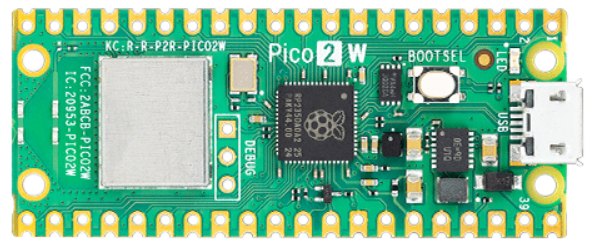
\includegraphics[width=10cm]{figuras/Pico_2w.png}\\
	\autoria{Adaptado de \citeonline{makerhero_pico2w}}
	\label{fig:01}
\end{figure}

Utiliza-se do microcontrolador RP2350, que é composto por um processador dual-core ARM Cortex-M33, operando em até 150 MHz. O componente conta com 520 KB de memória RAM e 4 MB de memória Flash integrada na placa. Além disso, o modelo oferece recursos avançados como unidade de ponto flutuante (FPU), tecnologia de segurança TrustZone, conexão Wi-Fi e Bluetooth 5.2, mantendo o suporte USB Host/Device e os modos de baixo consumo de energia (\textit{low power}). As principais especificações técnicas deste microcontrolador estão descritas no Quadro \ref{quadro:esp_pico2w}. 

A programação da placa pode ser realizada em MicroPython, C/C++ e Rust. O envio do código é feito na forma \textit{drag and drop} (arrastar e soltar), isto é, ao conectá-la ao computador, ela é reconhecida como um dispositivo de armazenamento (disco) onde o arquivo do código pode ser colocado para que a placa inicie a execução. A pinagem da placa Raspberry Pi Pico 2 W é apresentada na Figura \ref{fig:picow-pinout}.
\begin{figure}[!h]
    \centering
    \caption{Pinagem da placa Raspberry Pi Pico 2 W}
    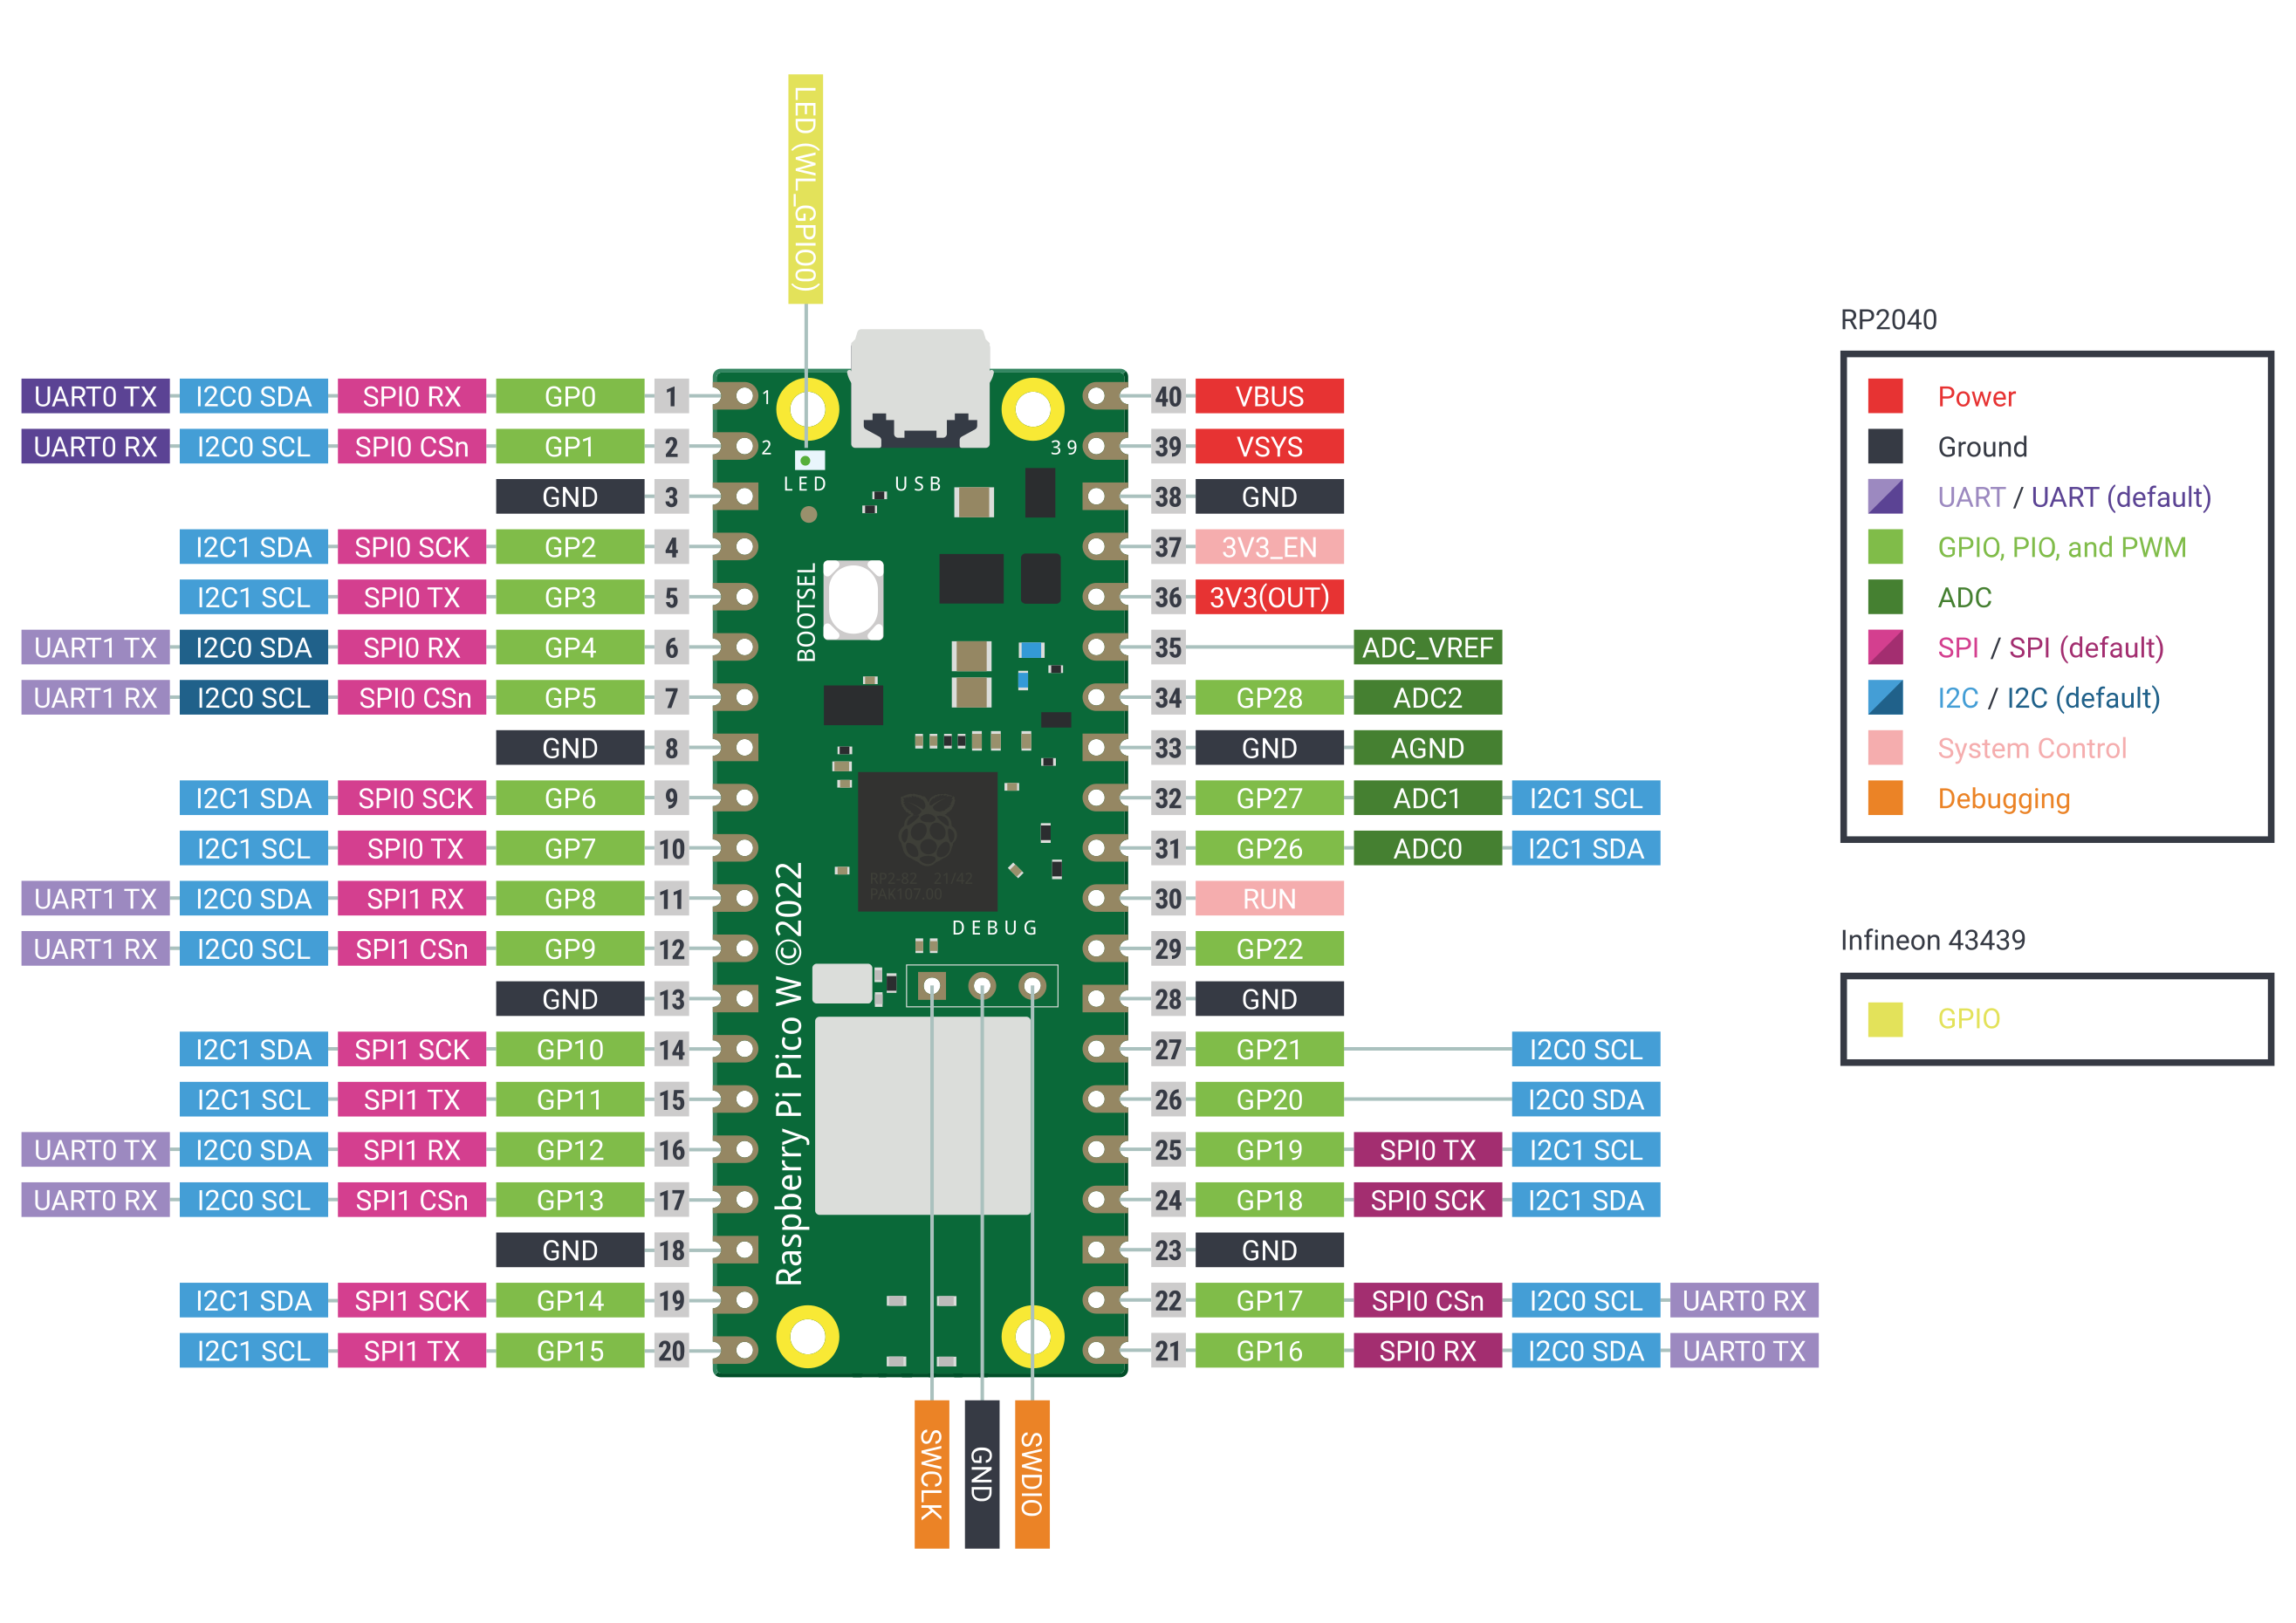
\includegraphics[width=12cm]{figuras/picow-pinout.png}\\
    \autoria{\cite{raspberrypi_pico_docs}}
    \label{fig:picow-pinout}

\end{figure}    
\begin{quadro}[htbp]
    \centering
    \caption{Especificações do Raspberry Pi Pico 2 W}
    \begin{tabular}{|l|l|}
    \hline
    \textbf{Tipo} & Microcontrolador \\ \hline
    \textbf{Fabricante} & Raspberry Pi Foundation \\ \hline
    \textbf{Preço} & R\$67,90 \\ \hline
    \textbf{Dimensões} & 51,3 mm $\times$ 21 mm $\times$ 3,9 mm \\ \hline
    \textbf{Software} & C/C++ SDK, MicroPython, Thonny IDE \\ \hline
    \textbf{Clock} & 150 MHz \\ \hline
    \textbf{Microcontrolador} & RP2350 (Dual-core ARM Cortex-M33) \\ \hline
    \textbf{Memória RAM} & 520 KB \\ \hline
    \textbf{Memória Flash} & 4 MB \\ \hline
    \textbf{GPIOs} & 26 GPIOs multifuncionais \\ \hline
    \textbf{Periféricos} & 2$\times$SPI, 2$\times$I2C, 2$\times$UART, 4$\times$ADC (12-bit), 24$\times$PWM \\ \hline
    \textbf{Wireless} & Infineon CYW43439 (Wi-Fi 2.4 GHz 802.11n) \\ \hline
    \textbf{Bluetooth} & Bluetooth 5.2 (BLE) \\ \hline
    \textbf{USB} & micro-USB \\ \hline
    \textbf{Tensão de Alimentação} & 1,8 V a 5,5 V (USB VBUS ou Externa) \\ \hline
    \textbf{Tensão de Operação} & 3,3 V \\ \hline
    \textbf{Miscelâneas} & Sensor de temperatura on-board, RTC de alta precisão \\ \hline
    \end{tabular}
    \autoria{Autoria Própria}
    \label{quadro:esp_pico2w}
\end{quadro}

\subsection{Sensor de corrente}
O SCT013-000 Figura \ref{fig:02} é um sensor de corrente não invasivo, amplamente utilizado para monitoramento de consumo energético. Ele é projetado para medir correntes alternadas (AC) em circuitos elétricos sem a necessidade de desconectar ou modificar a fiação existente. O sensor é composto por um transformador de corrente, que induz uma corrente proporcional à corrente primária que está sendo medida. 

O modelo SCT013-000 é capaz de medir correntes de até 100 A, com uma saída de tensão proporcional à corrente medida, facilitando a integração com sistemas de aquisição de dados. Para a medição da tensão de saida do sensor, é necessário o uso de um resistor de carga, que converte a corrente induzida em uma tensão mensurável pelo ADC do microcontrolador. As principais especificações técnicas deste sensor estão descritas no Quadro \ref{quadro:esp_SCT013}. 

\begin{figure}[!h]
	\centering
	\caption{Sensor de corrente SCT013-000}
	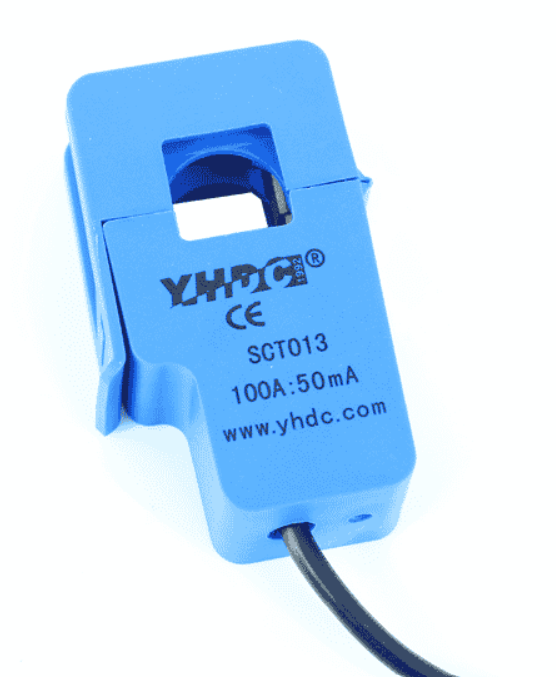
\includegraphics[width=10cm]{figuras/SCT013.png}\\
	\autoria{\cite{makerhero_sct013}}
	\label{fig:02}
\end{figure}


\begin{quadro}[htbp]
    \centering
    \caption{Especificações técnicas do sensor de corrente SCT-013-000}
    \begin{tabular}{|c|c|}
    \hline
    \textbf{Parâmetro} & \textbf{Especificação} \\ \hline
    Fabricante & YHDC \\ \hline
    Modelo & SCT-013-000 \\ \hline
    Tipo & Transformador de corrente (TC) não invasivo \\ \hline
    Corrente de entrada & 0 a 100 A AC \\ \hline
    Corrente de saída & 0 a 50 mA \\ \hline
    Relação de transformação & 2000:1 \\ \hline
    Tensão de saída & Definida pelo resistor de carga (burden) \\ \hline
    Precisão & ±1\% (típica) \\ \hline
    Linearidade & Alta dentro da faixa nominal \\ \hline
    Frequência de operação & 50 Hz a 60 Hz \\ \hline
    Isolamento & Isolação galvânica entre primário e secundário \\ \hline
    Rigidez dielétrica & Até 3 kV \\ \hline
    Tipo de instalação & Clamp (não invasivo) \\ \hline
    Diâmetro interno & Aproximadamente 13 mm \\ \hline
    Saída & Conector P2 (3,5 mm) \\ \hline
    Temperatura de operação & -25°C a 70°C \\ \hline
    Aplicações típicas & Monitoramento de energia, medição de carga \\ \hline
    \end{tabular}\\
    \autoria{Autoria Própria}
    \label{quadro:esp_SCT013}
\end{quadro}

\subsection{Sensor de Tensão}
O ZMPT101B presente na Figura \ref{fig:zmpt101b} é um sensor de tensão AC baseado em um transformador de alta precisão com relação de transformação de 1000:1000 e isolação galvânica de até 4 kV, garantindo segurança na medição direta da rede elétrica. O módulo é capaz de medir tensões AC na faixa de 0 a 250 V (50/60 Hz) com precisão de $\pm$3\% e linearidade de $\leq$0,2\%, fornecendo um sinal analógico proporcional à tensão medida com offset de VCC/2, compatível com conversores analógico-digitais de microcontroladores como Raspberry Pi e ESP32, a pinagem do módulo está ilustrada na Figura \ref{fig:zmpt_pinout}.

A amplitude da saída pode ser ajustada por meio de um potenciômetro multivolta \textit{onboard}, e o cálculo da tensão RMS é realizado via software, compensando o offset DC imposto pelo circuito de condicionamento baseado no amplificador operacional LM358. As principais especificações técnicas sobre o sensor ZMPT101B estão descritas no Quadro \ref{quad:zmpt101b}.

\begin{figure}[!h]
    \centering
    \caption{Pinagem do módulo ZMPT101B}
    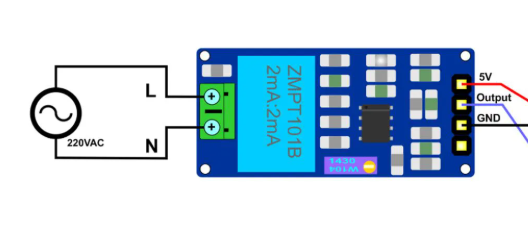
\includegraphics[width=10cm]{figuras/zmpt_pinout.png}\\
    \autoria{\cite{casa_da_robotica_zmpt101b}}
    \label{fig:zmpt_pinout}
\end{figure}


\begin{figure}[!h]
	\centering
	\caption{Sensor de tensão ZMPT101B}
	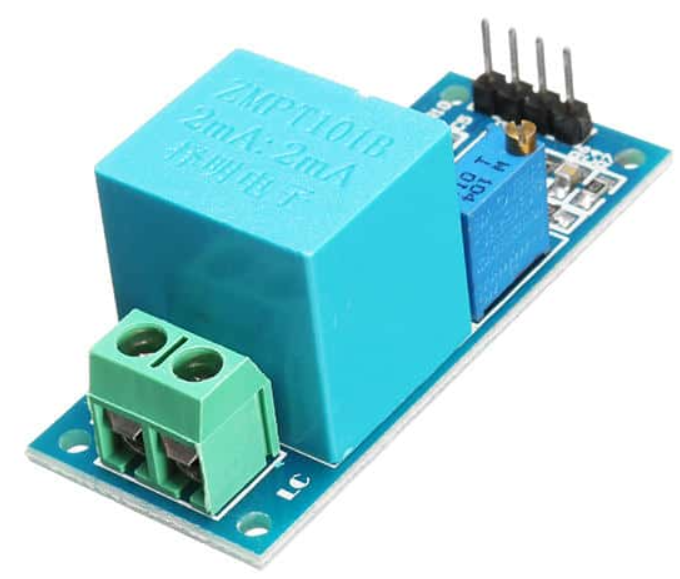
\includegraphics[width=10cm]{figuras/ZMPT101B.png}\\
	\autoria{\cite{casa_da_robotica_zmpt101b}}
	\label{fig:zmpt101b}
\end{figure}

\begin{quadro}[h]
\centering
\caption{Especificações técnicas do sensor de tensão ZMPT101B}
\begin{tabular}{|c|c|}
\hline
\textbf{Parâmetro} & \textbf{Especificação} \\
\hline
Fabricante & Qingxian Zeming Langxi Electronic \\
\hline
Modelo & ZMPT101B \\
\hline
Tipo & Transformador de tensão (TC) não invasivo \\
\hline
Tensão de entrada & 0 a 250 V AC \\
\hline
Corrente nominal & 2 mA (primário e secundário) \\
\hline
Relação de transformação & 1000:1000 \\
\hline
Tensão de saída & 0 a VCC (com offset de VCC/2) \\
\hline
Precisão & $\pm$3\% (típica) \\
\hline
Linearidade & $\leq$0,2\% (20\% a 120\% da carga nominal) \\
\hline
Erro de ângulo de fase & $\leq$20' (resistor de amostragem 100\,$\Omega$) \\
\hline
Frequência de operação & 50 Hz a 60 Hz \\
\hline
Isolamento & Isolação galvânica entre primário e secundário \\
\hline
Rigidez dielétrica & Até 4 kV \\
\hline
Tipo de instalação & Conexão direta em série (invasivo) \\
\hline
Alimentação do módulo & 5 V a 30 V DC \\
\hline
Saída & Sinal analógico (compatível com ADC) \\
\hline
Temperatura de operação & -20°C a 85°C \\
\hline
Aplicações típicas & Medição de tensão AC, monitoramento de energia \\
\hline
\end{tabular}\\
\label{quad:zmpt101b}
\autoria{Autoria Própria}
\end{quadro}

\subsection{Módulo MicroSD}
O módulo microSD é utilizado para realizar a leitura e gravação de dados em cartões de memória, sendo amplamente empregado em sistemas embarcados para armazenamento de informações. Ele apresenta compatibilidade com o Raspberry Pi Pico W e com bibliotecas disponíveis para esse microcontrolador, além de suportar cartões formatados em FAT32 com capacidade até de 2 GB e cartões micro SDHC (\textit{high-speed}) até 32 GB.

Seu circuito possui uma arquitetura simples, sendo baseado principalmente em um regulador de tensão integrado. Esse componente é responsável por converter a tensão de alimentação de entrada, que pode variar entre 3,3 V e 6 V, para uma tensão estável de 3,3 V, valor necessário para o funcionamento adequado dos cartões microSD.


\begin{figure}[!h]
	\centering
	\caption{Módulo MicroSD}
	\includegraphics[width=10cm]{figuras/MicroSD.png}\\
	\autoria{\cite{casadarobotica_modulosd}}
	\label{fig:microsd}
\end{figure}
\subsection{Módulo Multiplexador Analógico}

O módulo multiplexador analógico 74HC4067 é um circuito integrado CMOS de 16 canais utilizado para selecionar um entre diversos sinais analógicos ou digitais e direcioná-lo para uma única saída comum. Neste trabalho, sua utilização torna-se necessária devido à limitação do número de canais do conversor analógico-digital (ADC) disponível no microcontrolador Raspberry Pi Pico 2 W, permitindo a aquisição de múltiplos sinais provenientes dos sensores de corrente SCT013-000 e de tensão ZMPT101B utilizando apenas um canal de entrada analógica. A Figura \ref{fig:74HC4067} apresenta o módulo multiplexador analógico 74HC4067.

O funcionamento do módulo baseia-se na comutação eletrônica entre seus dezesseis canais de entrada (C0 a C15), realizada por meio de quatro linhas de seleção digitais (S0, S1, S2 e S3). Conforme a combinação lógica aplicada nessas entradas de controle, apenas um dos canais é conectado ao terminal comum (SIG), possibilitando que o microcontrolador realize a leitura sequencial dos sinais analógicos sem a necessidade de um conversor analógico-digital externo. Além disso, o módulo opera com baixa resistência de condução e reduzida corrente de fuga, características que contribuem para minimizar distorções durante a aquisição dos sinais.

As principais especificações técnicas do módulo multiplexador 74HC4067 estão descritas no Quadro \ref{quad:74HC4067}.
\begin{figure}[!h]
	\centering
	\caption{Módulo Multiplexador Analógico 74HC4067}
	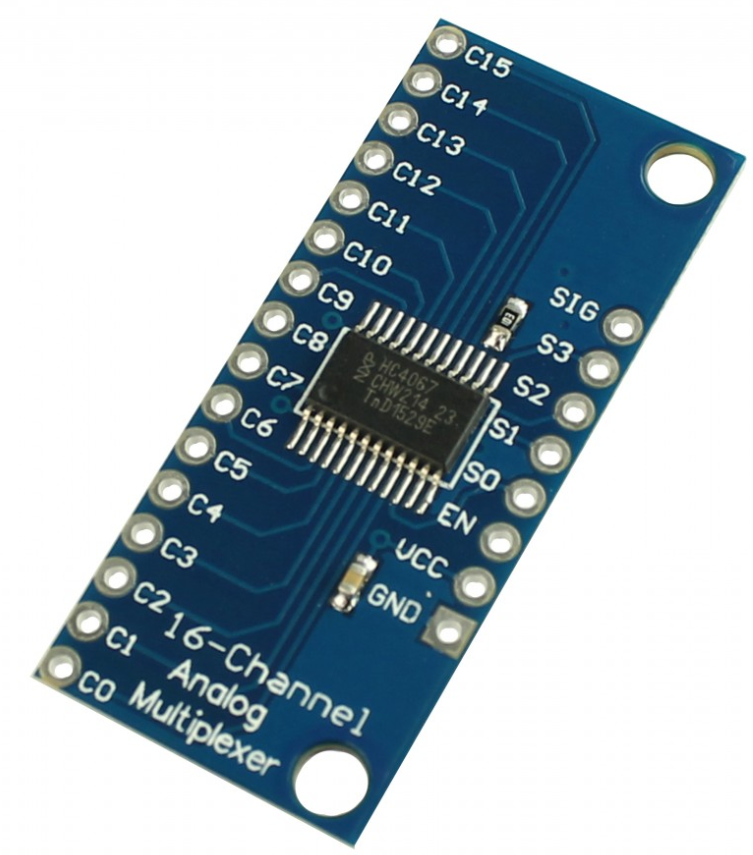
\includegraphics[width=8cm]{figuras/multiplexador.png}\\
	\autoria{\cite{usinainfo_multiplexador_74hc4067}}
	\label{fig:74HC4067}
\end{figure}


\begin{quadro}[h]
\centering
\caption{Especificações técnicas do módulo multiplexador analógico 74HC4067}
\label{quad:74HC4067}
\begin{tabular}{|p{6cm}|p{8cm}|}
\hline
\textbf{Parâmetro} & \textbf{Especificação} \\ \hline
Modelo & 74HC4067 \\ \hline
Tecnologia & CMOS \\ \hline
Tipo & Multiplexador/Demultiplexador analógico de 16 canais \\ \hline
Número de canais & 16 \\ \hline
Linhas de seleção & 4 (S0, S1, S2 e S3) \\ \hline
Canal comum & SIG \\ \hline
Tensão de alimentação & 2 V a 6 V \\ \hline
Tensão típica de operação & 3,3 V ou 5 V \\ \hline
Resistência ON típica & Aproximadamente 70 $\Omega$ (@ 4,5 V) \\ \hline
Corrente de fuga & Menor que 1 $\mu$A (típica) \\ \hline
Compatibilidade & Sinais analógicos e digitais \\ \hline
Aplicações típicas & Expansão de entradas ADC, seleção de sensores e aquisição de sinais \\ \hline
Encapsulamento & Módulo baseado no CI 74HC4067 (TSSOP-24/SOIC-24) \\ \hline
\end{tabular}
\caption*{Fonte: Autoria Própria.}
\end{quadro}





\subsection{Display OLED SSD1306}
O display OLED SSD1306 é um módulo de exibição baseado na tecnologia OLED (\textit{Organic Light-Emitting Diode}), que utiliza diodos orgânicos emissores de luz para gerar imagens. Ele é amplamente utilizado em projetos de eletrônica e sistemas embarcados devido à sua alta eficiência energética, contraste elevado e capacidade de exibir informações em tempo real. O módulo é compatível com o protocolo de comunicação I2C, permitindo uma interface simples e eficiente com microcontroladores como o Raspberry Pi Pico 2 W. 

A Figura \ref{fig:oled} apresenta o display OLED SSD1306, a pinagem do módulo, que é composta por quatro pinos: VCC (alimentação), GND, SCL (\textit{clock} do barramento I2C) e SDA (dados do barramento I2C). Devido a alta demanda de informações a serem exibidas, o sistema contará com botões de navegação para permitir a alternância entre diferentes telas de exibição, possibilitando ao usuário visualizar os dados de corrente, tensão e potência em tempo real, bem como o status do sistema.
\begin{figure}[!h]
	\centering
	\caption{Display SSD1306 OLED}
	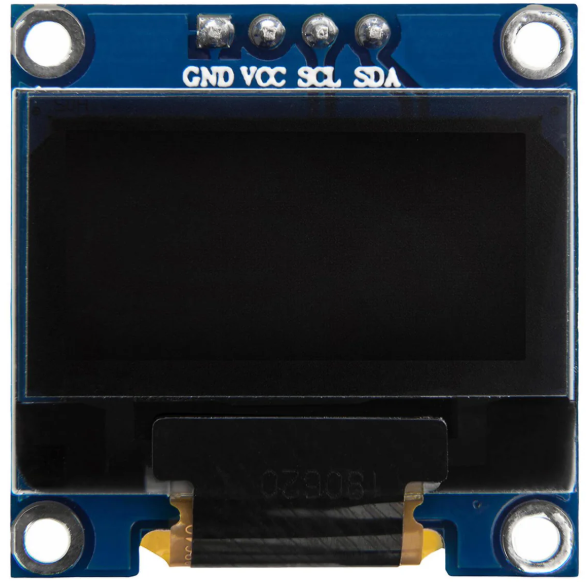
\includegraphics[width=8cm]{figuras/ssd1306.png}\\
	\autoria{\cite{azdelivery_oled}}
	\label{fig:oled}
\end{figure}
\section{Processamento Analógico do Sinal}
Com o propósito de adequar os sinais provenientes dos sensores SCT013-000, fez-se necessário o uso de condicionadores de sinais analógicos para converter o nível de corrente do sensor que varia de 0 a 50 mA em uma tensão compatível com o valor de referência do ADC do microcontrolador que é de 3,3V.

Para isso, foi utilizado um resistor de carga de 33 $\Omega$ em paralelo com o sensor, resultando em uma tensão máxima de 1,65 a 3,3V. Além disso, foi implementado um circuito de offset utilizando um divisor resistivo para elevar o nível de tensão do sinal para 1,65V, garantindo que o sinal esteja centrado em torno do ponto médio do ADC. A figura \ref{fig:condicionador_corrente} apresenta o diagrama do circuito de condicionamento de sinal para o sensor de corrente SCT013-000.
\begin{figure}[!h]
	\centering
	\caption{Condicionador de sinal para o sensor de corrente SCT013-000}
	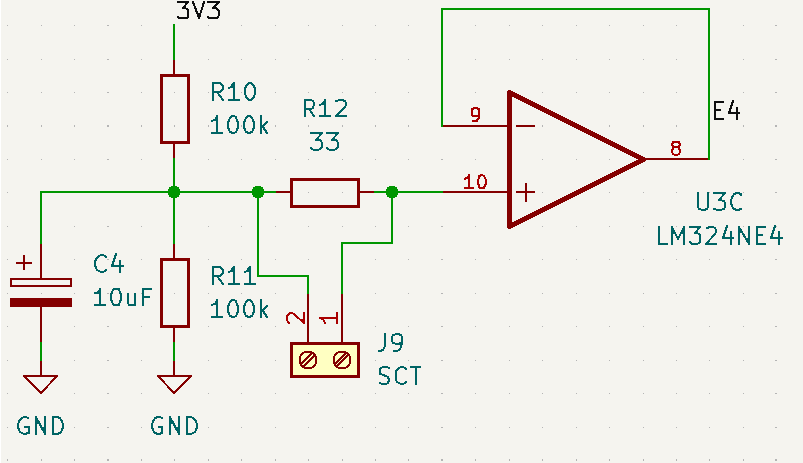
\includegraphics[width=10cm]{figuras/condicionador_sinais.png}\\
	\autoria{Autoria Própria}
	\label{fig:condicionador_corrente}
\end{figure}

Ademais, para atenuar os ruidosos provenientes da rede elétrica projetou-se um filtro passa-baixa de sétima ordem com frequência de corte de 300 Hz, por meio do \textit{software} FilterPro. A Figura \ref{fig:filtro} apresenta o diagrama do filtro passa-baixa implementado no sistema.

\begin{figure}[!h]
    \centering
    \caption{Filtro passa-baixa de sétima ordem com frequência de corte de 300 Hz}
    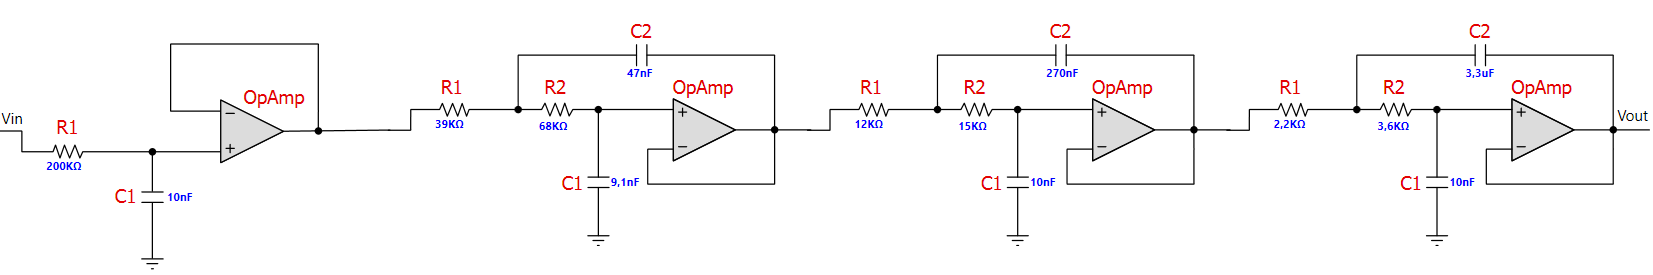
\includegraphics[width=17cm]{figuras/filtro.png}\\
    \autoria{Autoria Própria}
    \label{fig:filtro}
\end{figure}

Como forma de garantir a organização do circuito, os componentes foram montados em uma placa de circuito impresso (PCI) desenvolvida no \textit{software} KICAD, com o objetivo de reduzir o tamanho do sistema e facilitar a integração dos módulos. A Figura \ref{fig:pcb1} e Figura \ref{fig:pcb2} apresentam as placas de circuito impresso desenvolvida para o condicionamento dos sinais provenientes dos sensores e a Interface Homen Máquina(IHM). 
\begin{figure}[!h]
	\centering
	\caption{Placa de circuito impresso para condicionador e filtro}
	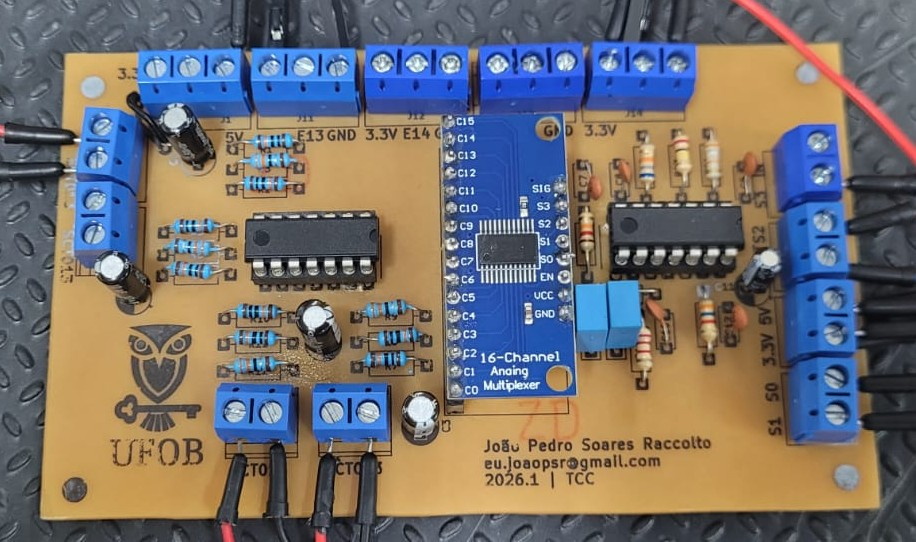
\includegraphics[width=10cm]{figuras/pcb2.jpeg}\\
	\autoria{Autoria Própria}
	\label{fig:pcb2}
\end{figure}

\begin{figure}[!h]
	\centering
	\caption{IHM}
	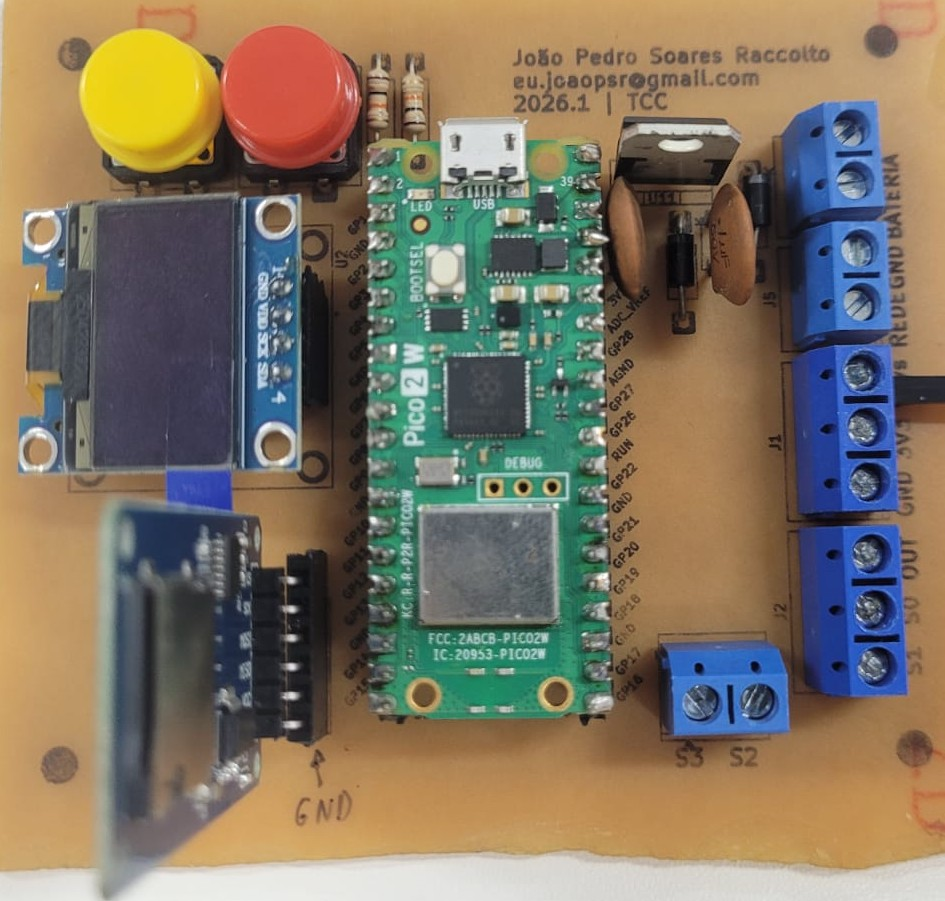
\includegraphics[width=10cm]{figuras/pcb1.jpeg}\\
	\autoria{Autoria Própria}
	\label{fig:pcb1}
\end{figure}

\section{Plataforma de Desenvolvimento}

O raspberry Pi Pico 2 W é uma placa de prototipagem baseada no microcontrolador RP2350, que oferece recursos avançados de conectividade sem fio, baixo consumo de energia e suporte a múltiplas linguagens de programação. A escolha dessa plataforma se deve à sua capacidade de atender às necessidades do sistema proposto, permitindo a aquisição, processamento e armazenamento dos dados elétricos de forma eficiente e confiável.

Entre as linguagens de programação destacam-se C/C++, empregada no desenvolvimento do firmware devido ao seu alto desempenho e controle direto sobre os periféricos do microcontrolador, e Python utilizado no desenvolvimento de scripts para processamento, análise e visualização dos dados coletados. Além disso, o RP2350 dispõe de interfaces de comunicação como UART, I²C, SPI, ADC e GPIO, possibilitando a integração com sensores, dispositivos de armazenamento e módulos de comunicação, tornando a plataforma adequada para aplicações de monitoramento e aquisição de dados em tempo real.

Nesse sentido, optou-se por utilizar a linguagem C/C++ para o desenvolvimento do \textit{firmware} utilizando como plataforma de desenvolvimento o \textit{software} Visual Studio Code, juntamente com a extensão Raspberry Pi Pico SDK, que fornece as bibliotecas e ferramentas necessárias para a programação do microcontrolador.

\section{Arquitetura do Firmware}



O firmware embarcado no Raspberry Pi Pico 2 W foi dividido em duas partes:
uma etapa de inicialização, executada apenas uma vez ao ligar o sistema, e
um laço principal, que se repete indefinidamente enquanto o equipamento
estiver energizado. Essa divisão foi adotada pois, a etapa de calibração
dos sensores depende de uma condição específica, ausência de carga nas
fases monitoradas que só é válida no instante da energização, enquanto
o restante do sistema precisa operar de forma contínua durante toda a
medição. A Figura~\ref{fig:fluxograma_firmware} apresenta o fluxograma
geral da lógica implementada no firmware.

Na inicialização, o microcontrolador configura os periféricos de hardware
necessários à aquisição dos sinais, isto é, o conversor analógico-digital
e o multiplexador CD74HC4067, além das entradas digitais usadas pelos
botões da interface física. Em seguida, é feita a calibração dos canais
de corrente e de tensão, em que o sistema mede o nível de offset CC e o
ruído de fundo de cada canal sem a presença de carga, valores que serão
usados posteriormente no cálculo do valor RMS de cada grandeza. Depois da
calibração, o firmware tenta sincronizar o relógio interno via NTP,
utilizando a conexão Wi-Fi da placa; caso essa sincronização falhe, o
sistema segue com um horário padrão, sem que isso impeça o restante da
inicialização. Por fim, é feita a tentativa de montagem do cartão
microSD, responsável por armazenar localmente os dados coletados. Se a
montagem falhar, o sistema continua funcionando normalmente, porém sem a
função de registro em arquivo, sinalizando esse estado ao usuário pela
interface.

Concluída a inicialização, o firmware passa a executar o laço principal,
que se repete em intervalos fixos de amostragem. A cada repetição:

\begin{enumerate}
    \item[I.] O estado dos botões de interface é verificado;

    \item[II.] Realiza-se a leitura sequencial dos canais de corrente
    (fases L1, L2 e L3) e do canal de tensão;

    \item[III.] Caso o instante de registro programado tenha sido
    atingido, os valores medidos são gravados em formato CSV no cartão
    microSD, caso contrário, essa etapa é ignorada e o firmware segue
    diretamente para a próxima;

    \item[IV.] O display OLED é atualizado com os valores instantâneos
    de corrente e tensão e com o estado atual do armazenamento;

    \item[V.] O firmware aguarda um intervalo de tempo fixo antes de
    reiniciar o ciclo a partir do item I.
\end{enumerate}

\begin{figure}[htb]
    \centering
    \caption{Fluxograma da lógica de funcionamento do firmware.}
    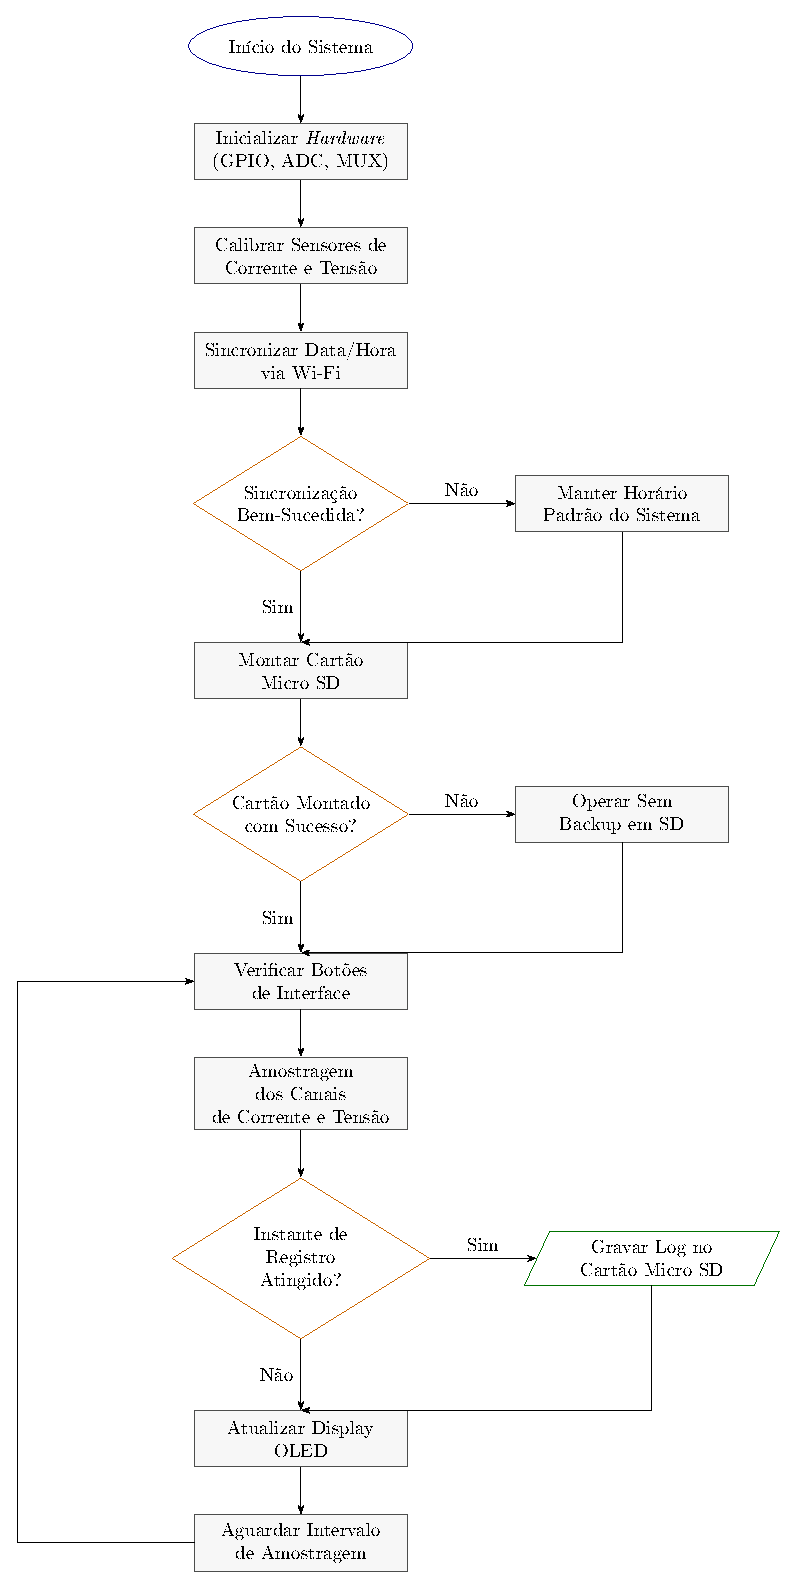
\includegraphics[width=0.55\textwidth]{figuras/fluxograma_clean.pdf}
    \label{fig:fluxograma_firmware}\\
    \autoria{Autoria Própria.}
\end{figure}

O uso de interrupção para o tratamento dos botões, em vez de varredura,
foi necessário porque o tempo de execução da etapa de amostragem dos
canais é da ordem de segundos, o que faria com que o acionamento de um
botão fosse perdido caso dependesse de ser lido dentro do próprio laço de
medição.
